\documentclass{letask}

\begin{document}
\begin{titlepage}
\center % Center everything on the page
 
%----------------------------------------------------------------------------------------
%	HEADING SECTIONS
%----------------------------------------------------------------------------------------

\textsc{\LARGE Московский\\[-0.2cm]Физико-Технический Институт\\[0.1cm]\large (государственный университет)}\\[1.5cm] % Name of your university/college
\textsc{\Large Кафедра общей физики}\\[0.1cm] % Major heading such as course name
\textsc{\large Лабораторная работа \textnumero  4.4.1}\\[0.5cm] % Minor heading such as course title

%----------------------------------------------------------------------------------------
%	TITLE SECTION
%----------------------------------------------------------------------------------------

\HRule
\\[0.4cm]
{ \huge \bfseries Амплитудная\\[0.2cm]
дифракционная решетка}
\\[0.6cm] % Title of your document
\HRule
\\[1.5cm]


 
%----------------------------------------------------------------------------------------
%	AUTHOR SECTION
%----------------------------------------------------------------------------------------

\begin{minipage}{0.4\textwidth}
	\begin{flushleft} \large
		\textsf{Студент}
		
		Ришат \textsc{Исхаков} \\[-0.15cm]
		513 группа
	\end{flushleft}
\end{minipage}
~
\begin{minipage}{0.4\textwidth}
	\begin{flushright} \large
		\textsf{Преподаватель}
		
		Александр Александрович \\[-0.15cm]
		\textsc{Казимиров} % Supervisor's Name
	\end{flushright}
\end{minipage}

\begin{bottompar}
	\begin{center}
		
\includegraphics[width = 80 mm]{logo.jpg}
	\end{center}
	{\large \today}

\end{bottompar}
\vfill % Fill the rest of the page with whitespace

\end{titlepage}

\textbf{Цель работы:} знакомство с работой и настройкой гониометра Г5, определение спектральных характеристик амплитудной решетки.

\textbf{В работе используются:} гониометр, дифракционная решетка, ртутная лампа.

\section{Теоретическая часть}

Амплитудную решетку можно представить в виде непрозрачного экрана, в котором прорезано большое число $N$ параллельных щелей - штрихов, расстояние между которыми $d$ (период решетки).


Пусть на решетку падает излучение с длиной волны $\lambda$ по нормали к плоскости решетки. Вследствие дифракции лучи, прошедшие через щель в решетке, отклоняются от своего первоначального направления. Рассмотрим лучи, отклонившиеся на угол $\varphi$. Разность хода лучей о эквивалентных точек двух соседних штрихов равна 
\[ \Delta = d \sin \varphi .\]

Если эта величина равна целому числу длин волны:
\[ d \sin \varphi = m \lambda, \quad m = 0, \pm 1, \pm 2, ... ,\]
то волны взаимно усиливают друг друга.


В соответствии с принципом Гюйгенса–Френеля распределение интенсивности в дифракционной картине определяется суперпозицией волн, приходящих в точку наблюдения от различных щелей решётки. При этом амплитуды всех интерферирующих волн при заданном угле $\varphi$ практически одинаковы, а фазы составляют арифметическую прогрессию.


\[
I = I_0 \dfrac{sin^2[N(kd \sin{\varphi})/2]}{sin^2[(kd \sin{\varphi})/2]},
\]

где $k$~--~волновое число, $I_0$~--~интенсивность волны, идущей от одного штриха. При большом числе щелей свет, прошедший через решётку, распространяется по ряду резко ограниченных направлений. Если на дифракционную решётку падает свет сложного спектрального состава, то после решётки образуется спектр, причём фиолетовые лучи отклоняются решёткой меньше, чем красные (чем больше длина волны, тем сильнее лучи отклоняются решеткой). Входящая в величина $m$ носит название порядка спектра. При $m = 0$ максимумы интенсивности для всех длин волн располагаются при $\varphi = 0$ и накладываются друг на друга. При освещении белым светом нулевой максимум, в отличие от всех прочих, оказывается поэтому неокрашенным. Спектры первого, второго и т.д. порядков располагаются симметрично по обе стороны от нулевого.



\textbf{Угловая дисперсия} $D$ характеризует угловое расстояние $d \varphi$ между спектральными линиями, отстоящими по длине волны на $d \lambda$:
\[
D=\dfrac{d \varphi}{d \lambda}=\frac{m}{d cos \varphi}=\dfrac{m}{\sqrt{d^{2}-(m \lambda)^{2}}}
\]

\textbf{Разрешающая способность дифракционной решетки.} Возможность разрешения двух близких спектральных линий зависит от их ширины и от расстояния между ними. Угловое расстояние между двумя близкими спектральными компонентами с длинами волн $\lambda$ и ($\lambda + \Delta \lambda$) равно:
\[
\Delta \varphi =  D d \lambda = \frac{m \Delta \lambda}{d \cos{\varphi}} 
\]

Согласно критерию Рэлея линии становятся неразличимыми, когда расстояние между ними меньше, чем расстояние от максимума одной линии до её первого минимума. Пусть решетка имеет $N$ штрихов. Выберем главный максимум $m$-го порядка для компоненты $\lambda$. Направление на первый дифракционный минимум дается равенством 
\[ d \sin \varphi = \left( m + \dfrac{1}{N} \right) \lambda. \]
По критерию Рэлея это же направление должно соответствовать главному дифракционному максимуму для второй компоненты $\lambda + \Delta \lambda$:
\[ d \sin \varphi = m (\lambda + \Delta \lambda) .\]

Из последних двух равенств находим 
\[\Delta \lambda = \dfrac{\lambda}{mN}.\]
По определению разрешающая способность спектрального прибора $R = \lambda / \Delta \lambda$~--~это отношение длины волны к разности длин волн двух линий, разрешаемых по критерию Рэлея.

Таким образом, приходим к следующему выражению для разрешающей способности дифракционной решетки:
\[R = \lambda / \Delta \lambda = mN\]

\section{Установка для измерений}

Исследование спектра ртутной лампы, определение периода и спектральных характеристик решетки проводится с помощью гониометра Г5.

\begin{figure}[H]
\centering
	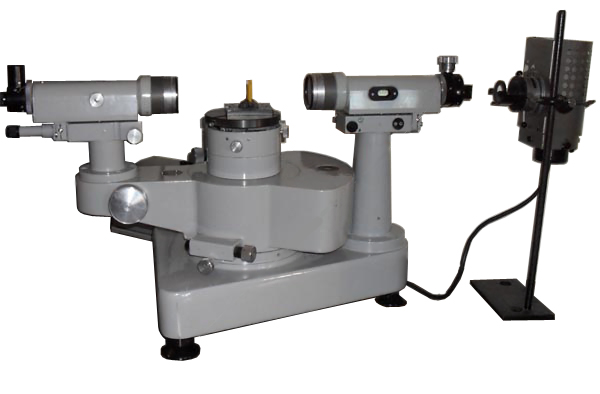
\includegraphics[width = 0.7\lw]{g5}
	\caption{Внешний вид гониометра Г5}
	\label{fig:g5}
\end{figure}


\begin{figure}[H]
\centering
	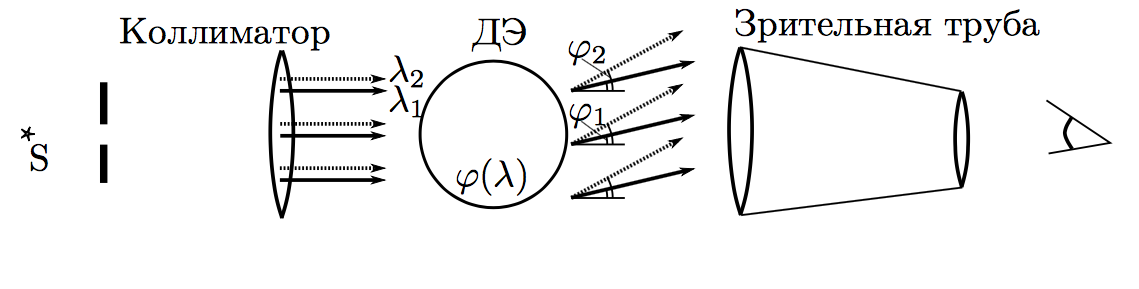
\includegraphics[width = \lw]{scheme}
	\caption{Схема прибора: источник-коллиматор -- диспергирующий элемент -- зрительная труба}
	\label{fig:scheme}
\end{figure}

\section{Измерения}



\section{Вывод}
Мы исследовали явления дифракции Френеля и Фраунгофера на щели, посчитали ширину щели теоретически и экспериментально.
\end{document}
